\documentclass[12pt,a4paper]{article}
% Compiler: pdfLaTeX (Overleaf default)
\usepackage[T2A,T1]{fontenc}
\usepackage[utf8]{inputenc}
\usepackage[russian,english]{babel}
\usepackage[a4paper,left=3cm,right=1.5cm,top=2cm,bottom=2cm]{geometry}
\usepackage[expansion=false]{microtype}
\usepackage{setspace}
\onehalfspacing
\usepackage{amssymb}
\usepackage{pifont}
\usepackage{wasysym}
\usepackage{array}
\usepackage{tabularx}
\usepackage{xltabular}
\usepackage{booktabs}
\usepackage[table]{xcolor}
\usepackage{caption}
\captionsetup{font=small,labelfont=bf,justification=raggedright,singlelinecheck=false}
\captionsetup[table]{position=top,skip=4pt}
\usepackage{enumitem}
\setlist{nosep,leftmargin=1.6em}
\usepackage[nobottomtitles*]{titlesec}
\renewcommand{\bottomtitlespace}{0.15\textheight}
\titleformat{\section}{\large\bfseries}{\thesection.}{0.6em}{}
\titleformat{\subsection}{\normalsize\bfseries}{\thesubsection.}{0.6em}{}
\titlespacing*{\section}{0pt}{1.2em}{0.5em}
\titlespacing*{\subsection}{0pt}{0.9em}{0.4em}
\usepackage{needspace}
\usepackage{etoolbox}
\usepackage{fancyhdr}
\pagestyle{fancy}\fancyhf{}
\fancyfoot[C]{\thepage}
\renewcommand{\headrulewidth}{0pt}
\usepackage{xurl}
\usepackage[colorlinks=true,linkcolor=black,citecolor=blue!50!black,urlcolor=blue!50!black]{hyperref}
\setlength{\parindent}{1.25cm}
\setlength{\parskip}{0pt}
\setlength{\emergencystretch}{3em}
\urlstyle{same}

% table style
\definecolor{headgray}{gray}{0.90}
\definecolor{linegray}{gray}{0.70}
\newcolumntype{L}{>{\raggedright\arraybackslash}X}
\newcolumntype{P}[1]{>{\raggedright\arraybackslash}p{#1}}
\newcolumntype{C}[1]{>{\centering\arraybackslash}p{#1}}
\newcommand{\rl}{\arrayrulecolor{linegray}\hline\arrayrulecolor{black}}
\newcommand{\thead}{\rowcolor{headgray}}

% comparison marks
\newcommand{\yes}{\ensuremath{\checkmark}}
\newcommand{\no}{\ding{55}}
\newcommand{\partly}{\LEFTcircle}
\newcommand{\ru}[1]{\foreignlanguage{russian}{#1}}
\newcommand{\doi}[1]{doi: \href{https://doi.org/#1}{#1}}

% title page
\newcommand{\maketitlepage}[1]{%
\begin{titlepage}
\centering
{\large Astana IT University\par}
{\normalsize School of Software Engineering\par}
\vspace{4.5cm}
{\normalsize Diploma Project\par}
\vspace{0.6cm}
{\Large\bfseries Development of a System for Detecting and Anonymizing Personal Data Before Sending Text to Artificial Intelligence Services\par}
\vspace{1.2cm}
{\LARGE #1\par}
\vfill
\begin{flushright}
\begin{tabular}{@{}l@{}}
\textbf{Authors:} Dossan Amina, Abzhamal Nazerke\\
\textbf{Educational programme:} Software Engineering\\
\textbf{Supervisor:} Sakhipov A.A., PhD,\\ \hspace{2.2cm}Assistant Professor
\end{tabular}
\end{flushright}
\vspace{2.5cm}
{\normalsize Astana, 2026\par}
\end{titlepage}
\setcounter{page}{2}}
\usepackage{graphicx}
\usepackage{float}
\graphicspath{{diagrams/}{../../diagrams/}}
\begin{document}
\maketitlepage{System Design Diagrams}

\tableofcontents
\newpage

\section{Introduction}

This document presents the design diagrams of the PII Anonymization Gateway: the architecture diagram, the sequence diagram of the main scenario, the use case diagram and the entity-relationship (ER) diagram of the database. The diagrams are based on the documents \emph{Requirements Specification} and \emph{Technology Comparison} and are consistent with the user interface prototype. The editable sources (\texttt{.drawio}) and the exported images (\texttt{.png}) are stored in the \texttt{diagrams} directory of the project repository.

\section{Architecture}

Figure~\ref{fig:arch} shows the components of the system and their deployment. All components that process original personal data are deployed within the organization's infrastructure using Docker Compose (NFR-3); only anonymized text crosses the boundary of the organization (NFR-2).

\begin{figure}[H]
\centering
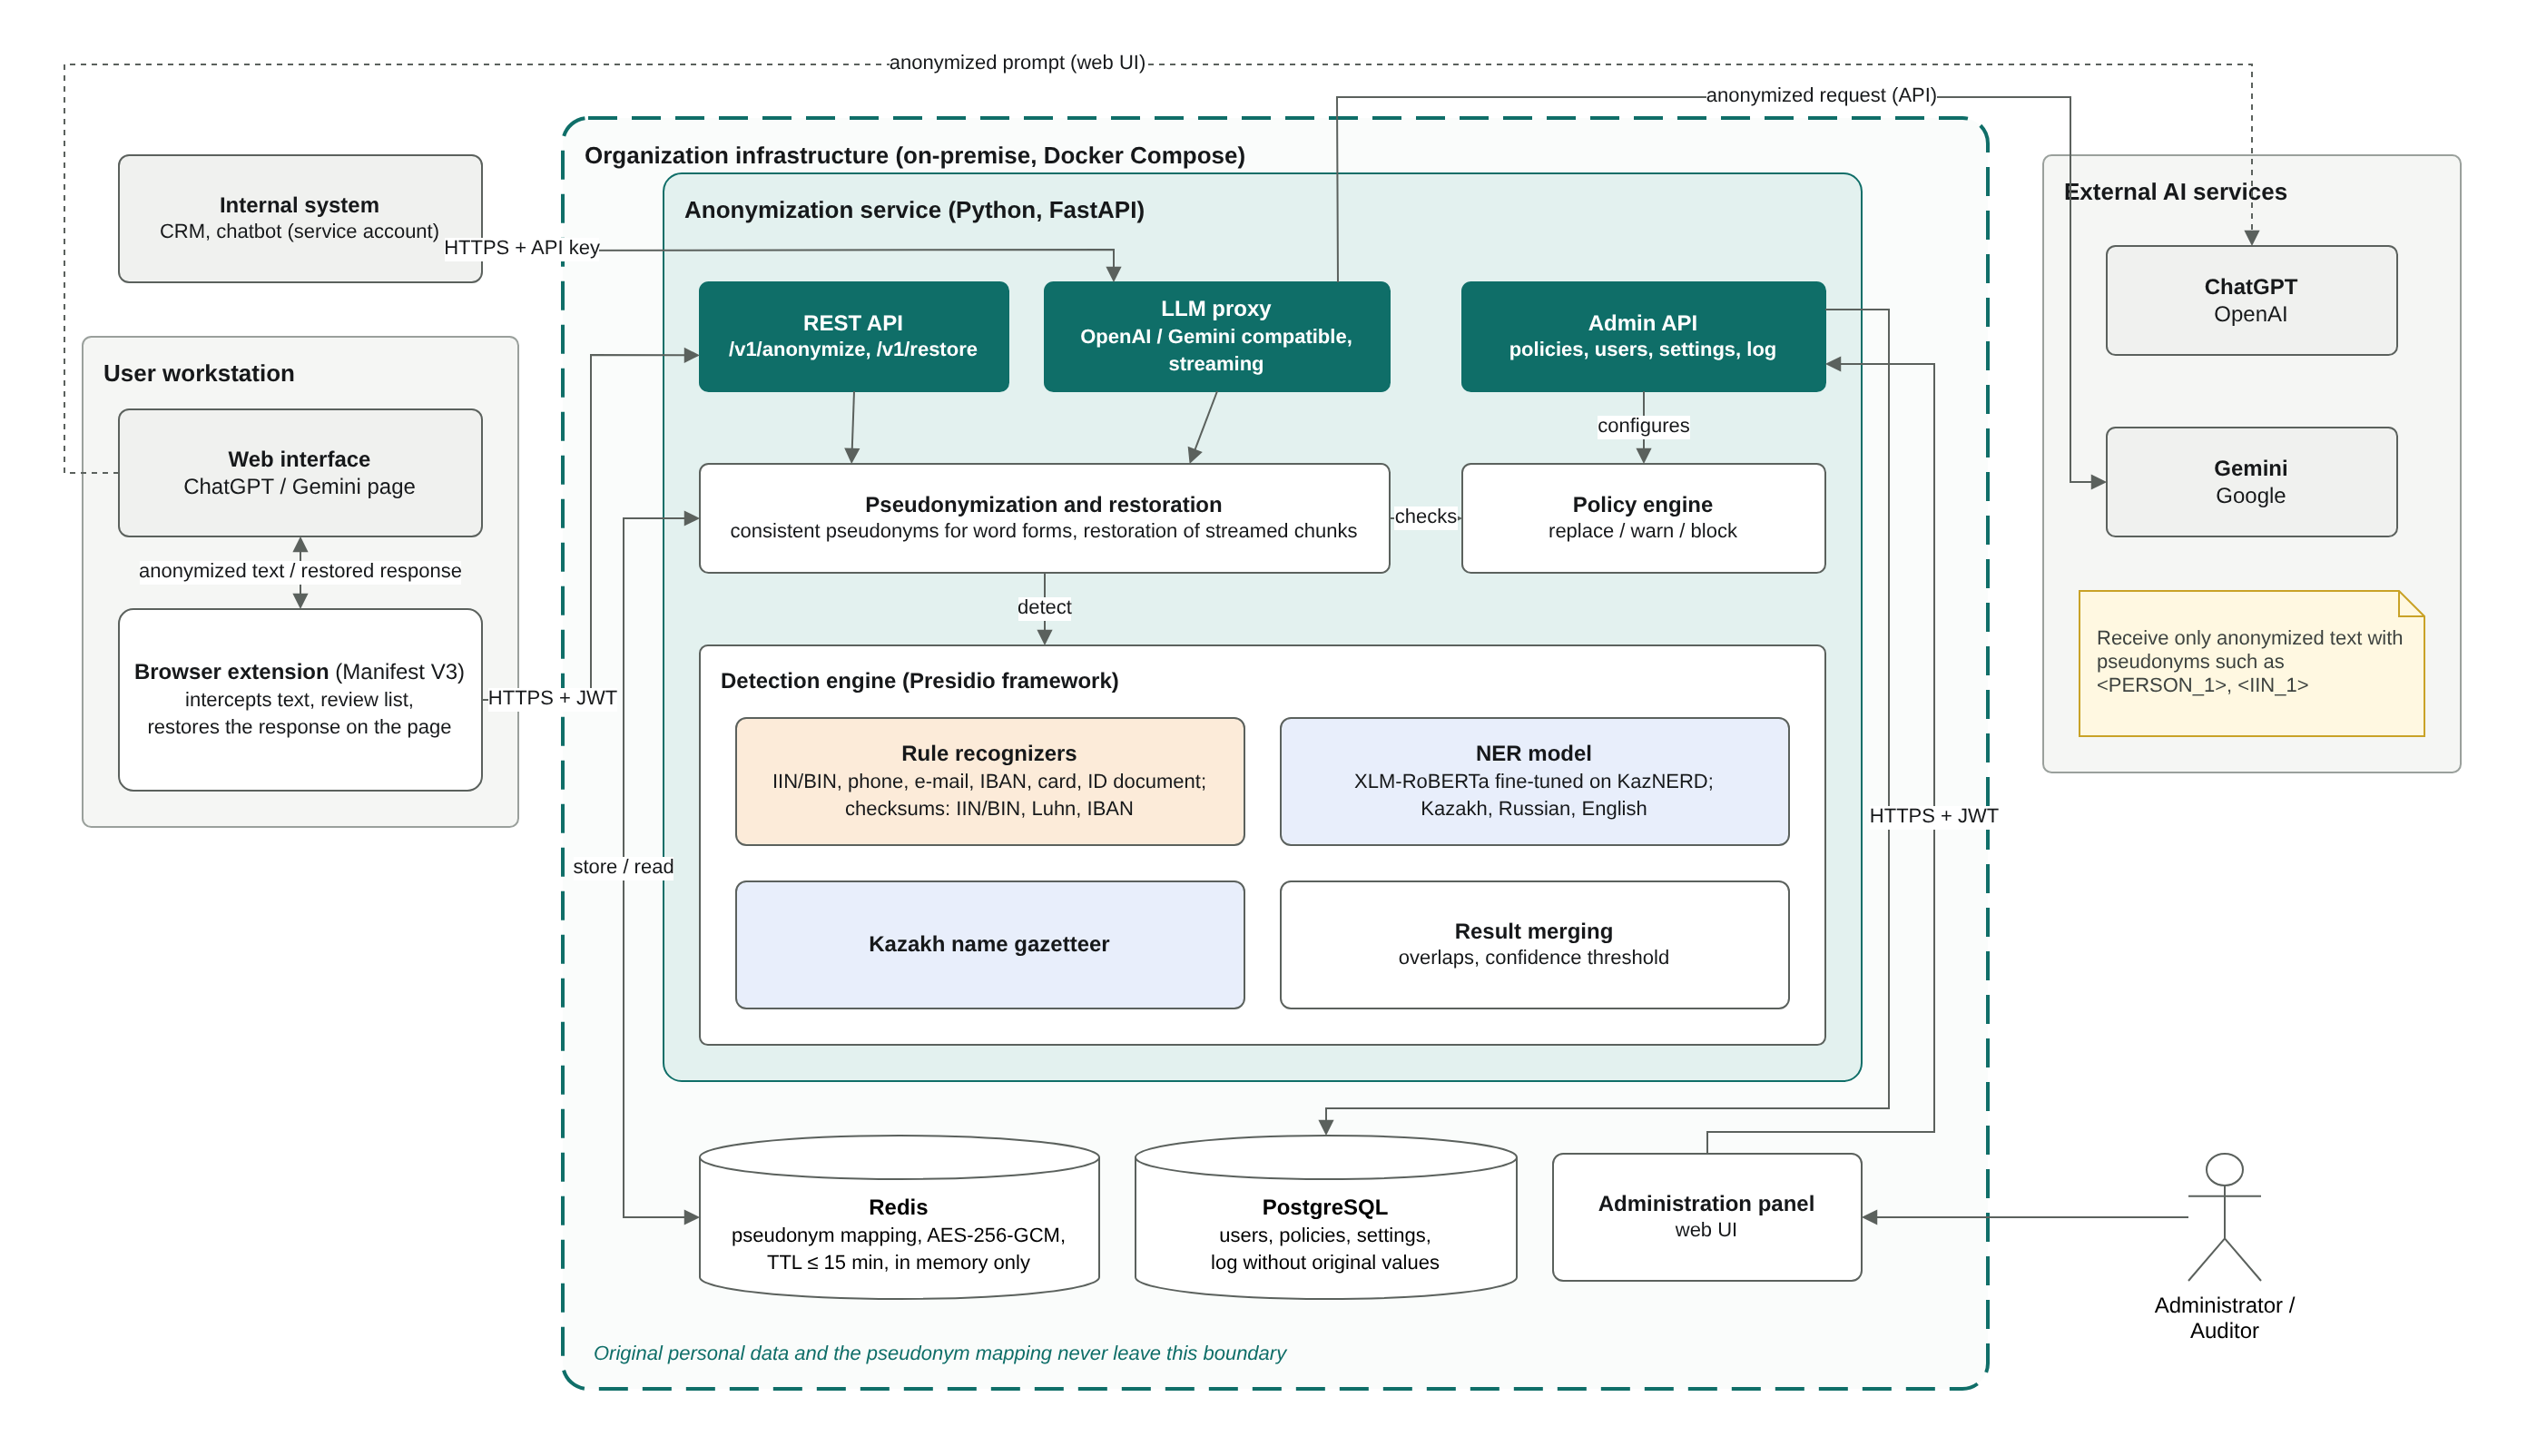
\includegraphics[width=\linewidth]{architecture.png}
\caption{Architecture of the system}\label{fig:arch}
\end{figure}

The system consists of the following components:
\begin{itemize}
\item \emph{Browser extension} (Manifest V3) intercepts the text in the web interfaces of ChatGPT and Gemini, sends it to the anonymization service, shows the detected data for review and restores the response on the page (FR-5).
\item \emph{Anonymization service} (Python, FastAPI) provides three interfaces: the REST API for the extension, the LLM proxy compatible with the OpenAI and Gemini interfaces for service accounts (FR-8), and the Admin API for the administration panel.
\item \emph{Detection engine} is built on the Presidio framework and combines rule recognizers with checksum validation, the XLM-RoBERTa NER model fine-tuned on KazNERD and the Kazakh name gazetteer; the results are merged using the confidence threshold (FR-1, FR-2).
\item \emph{Pseudonymization and restoration module} assigns consistent pseudonyms and restores original values, including streamed responses (FR-3, FR-4); the \emph{policy engine} applies the actions replace, warn and block (FR-6).
\item \emph{Redis} stores the pseudonym mapping in memory, encrypted with AES-256-GCM, with a retention of at most 15 minutes (NFR-2).
\item \emph{PostgreSQL} stores users, roles, policies, settings and the log without original values (FR-7).
\item \emph{Administration panel} is a web interface for administrators and auditors (FR-7).
\end{itemize}

\section{Sequence of the Main Scenario}

Figure~\ref{fig:seq} shows the interaction of the components when a user sends a request containing personal data through the browser extension and receives a restored response (use cases UC-1 and UC-2).

\begin{figure}[H]
\centering
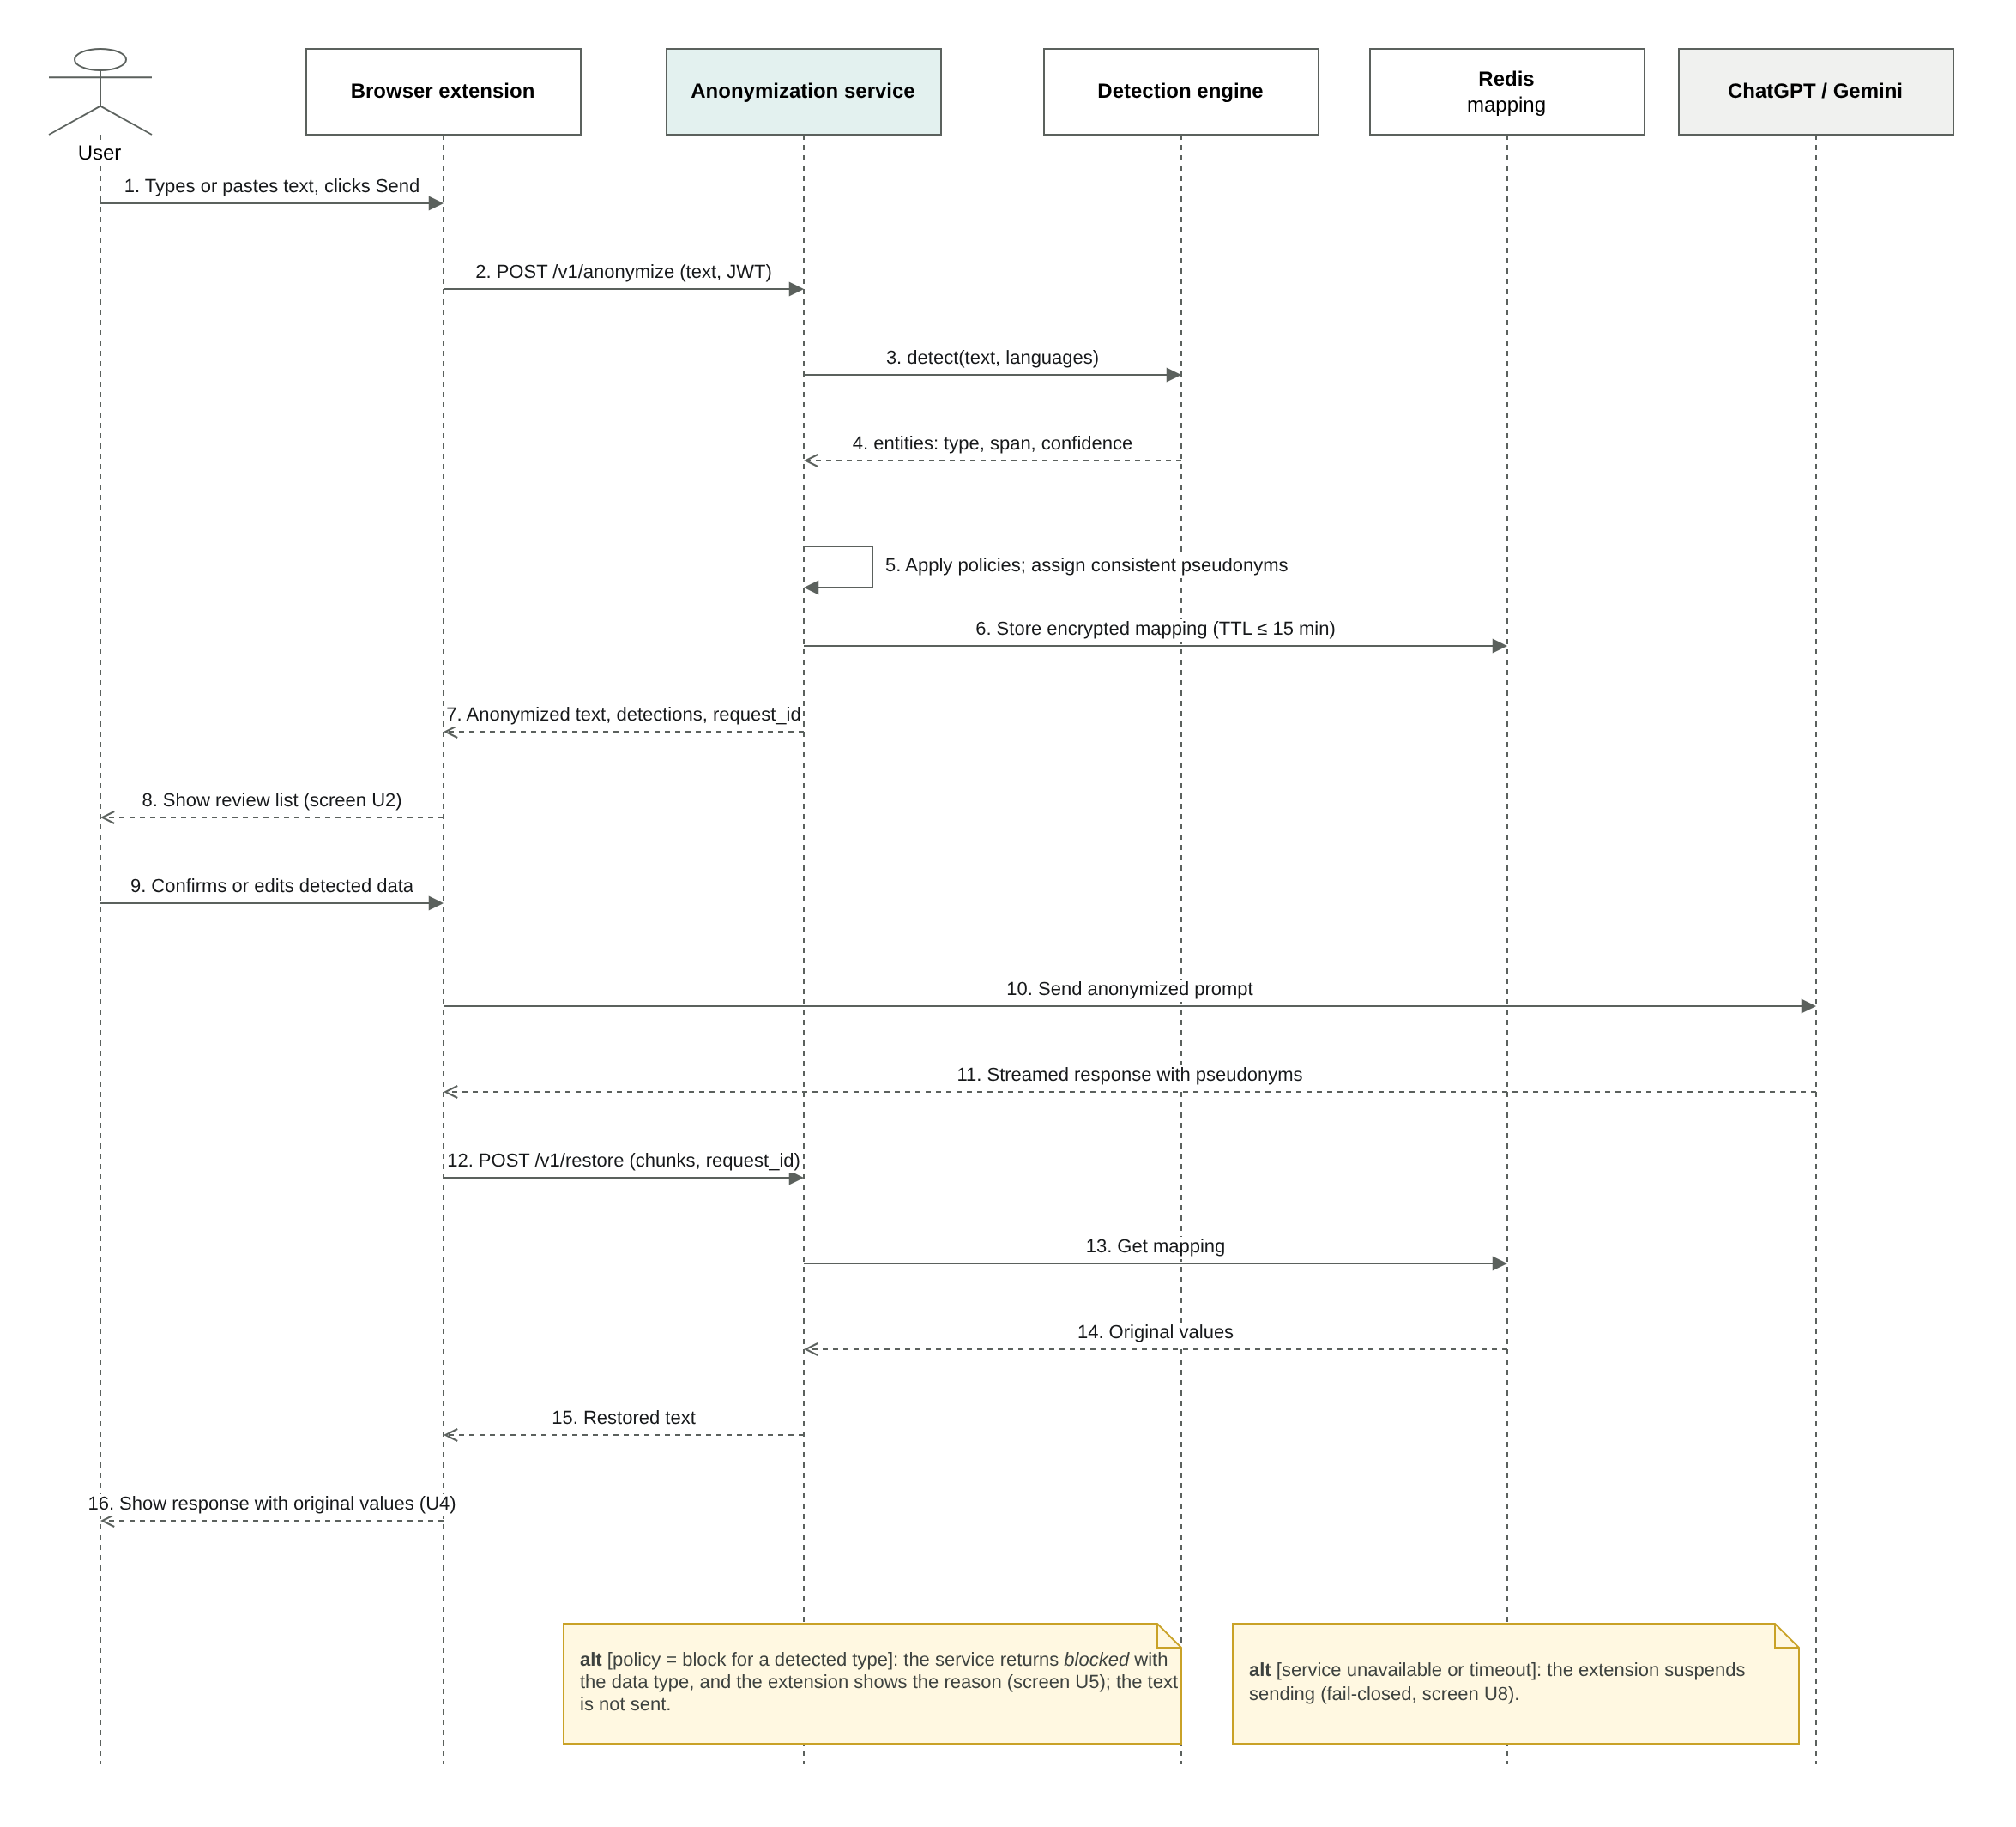
\includegraphics[width=\linewidth]{sequence.png}
\caption{Sequence diagram of sending a request and restoring the response}\label{fig:seq}
\end{figure}

The original text is sent only to the anonymization service within the organization (step 2). The AI service receives only the anonymized text (step 10), and the original values are restored using the mapping stored in Redis (steps 12--15). If a detected data type has the policy ``block'', the text is not sent and the user sees the reason; if the anonymization service is unavailable, sending is suspended (NFR-4).

\section{Use Cases}

Figure~\ref{fig:uc} shows the actors of the system and the main use cases defined in the requirements specification.

\begin{figure}[H]
\centering
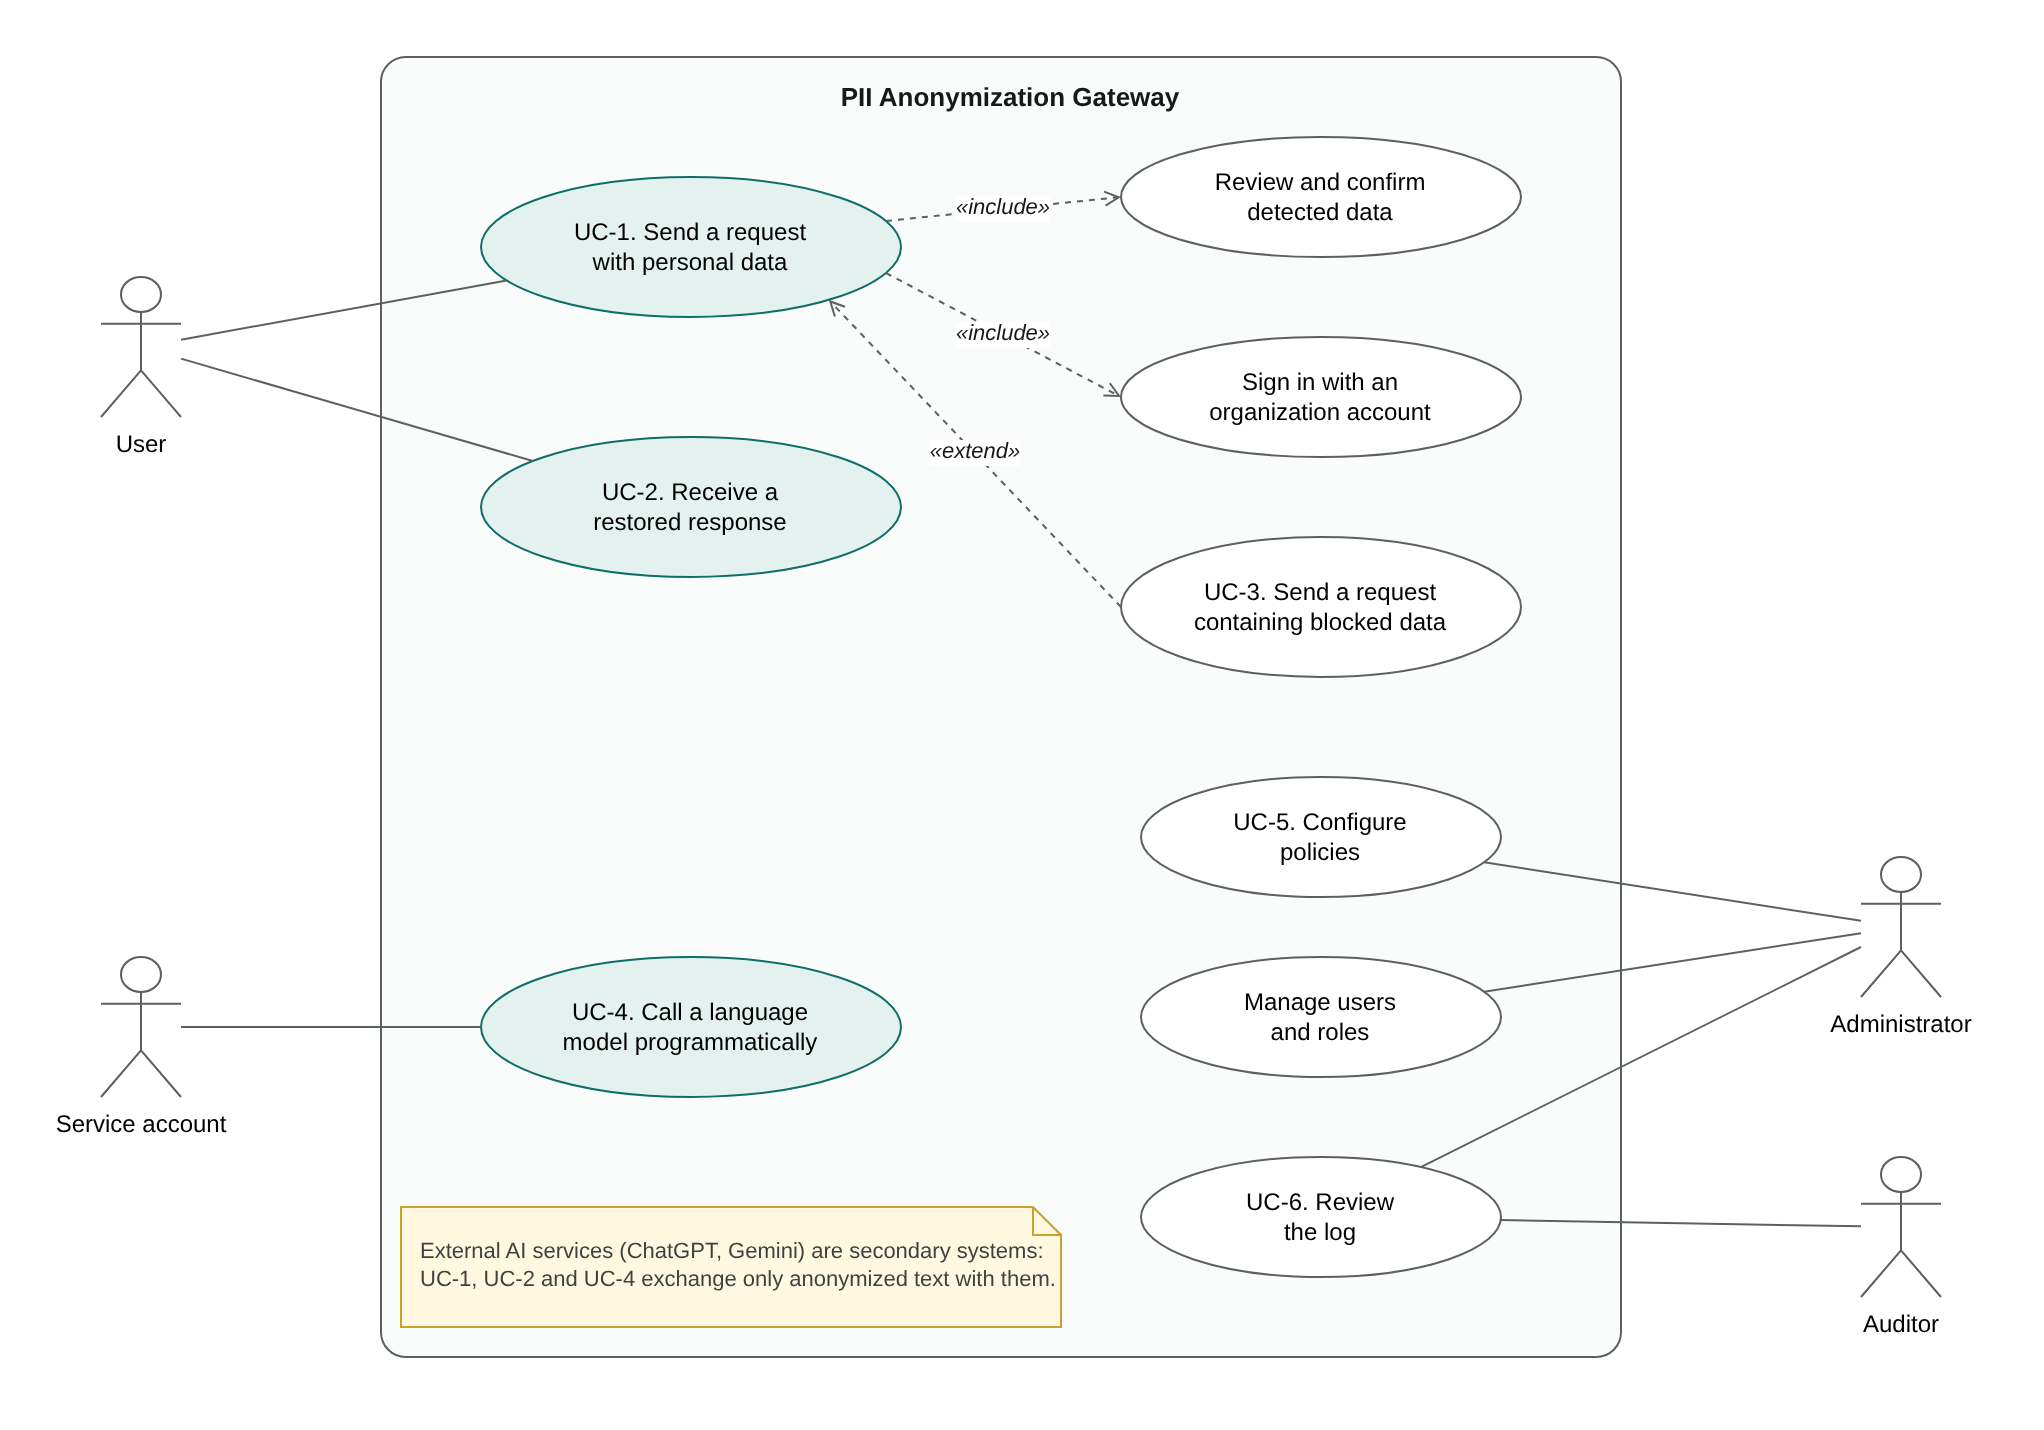
\includegraphics[width=0.92\linewidth]{use-case.png}
\caption{Use case diagram}\label{fig:uc}
\end{figure}

The user sends requests and receives restored responses (UC-1, UC-2); reviewing the detected data and signing in with an organization account are included in UC-1, and sending a request with blocked data (UC-3) extends it. The service account calls a language model through the API proxy (UC-4). The administrator configures policies, manages users and roles and reviews the log (UC-5, UC-6); the auditor has read-only access to the log.

\section{Database}

Figure~\ref{fig:er} shows the structure of the PostgreSQL database.

\begin{figure}[H]
\centering
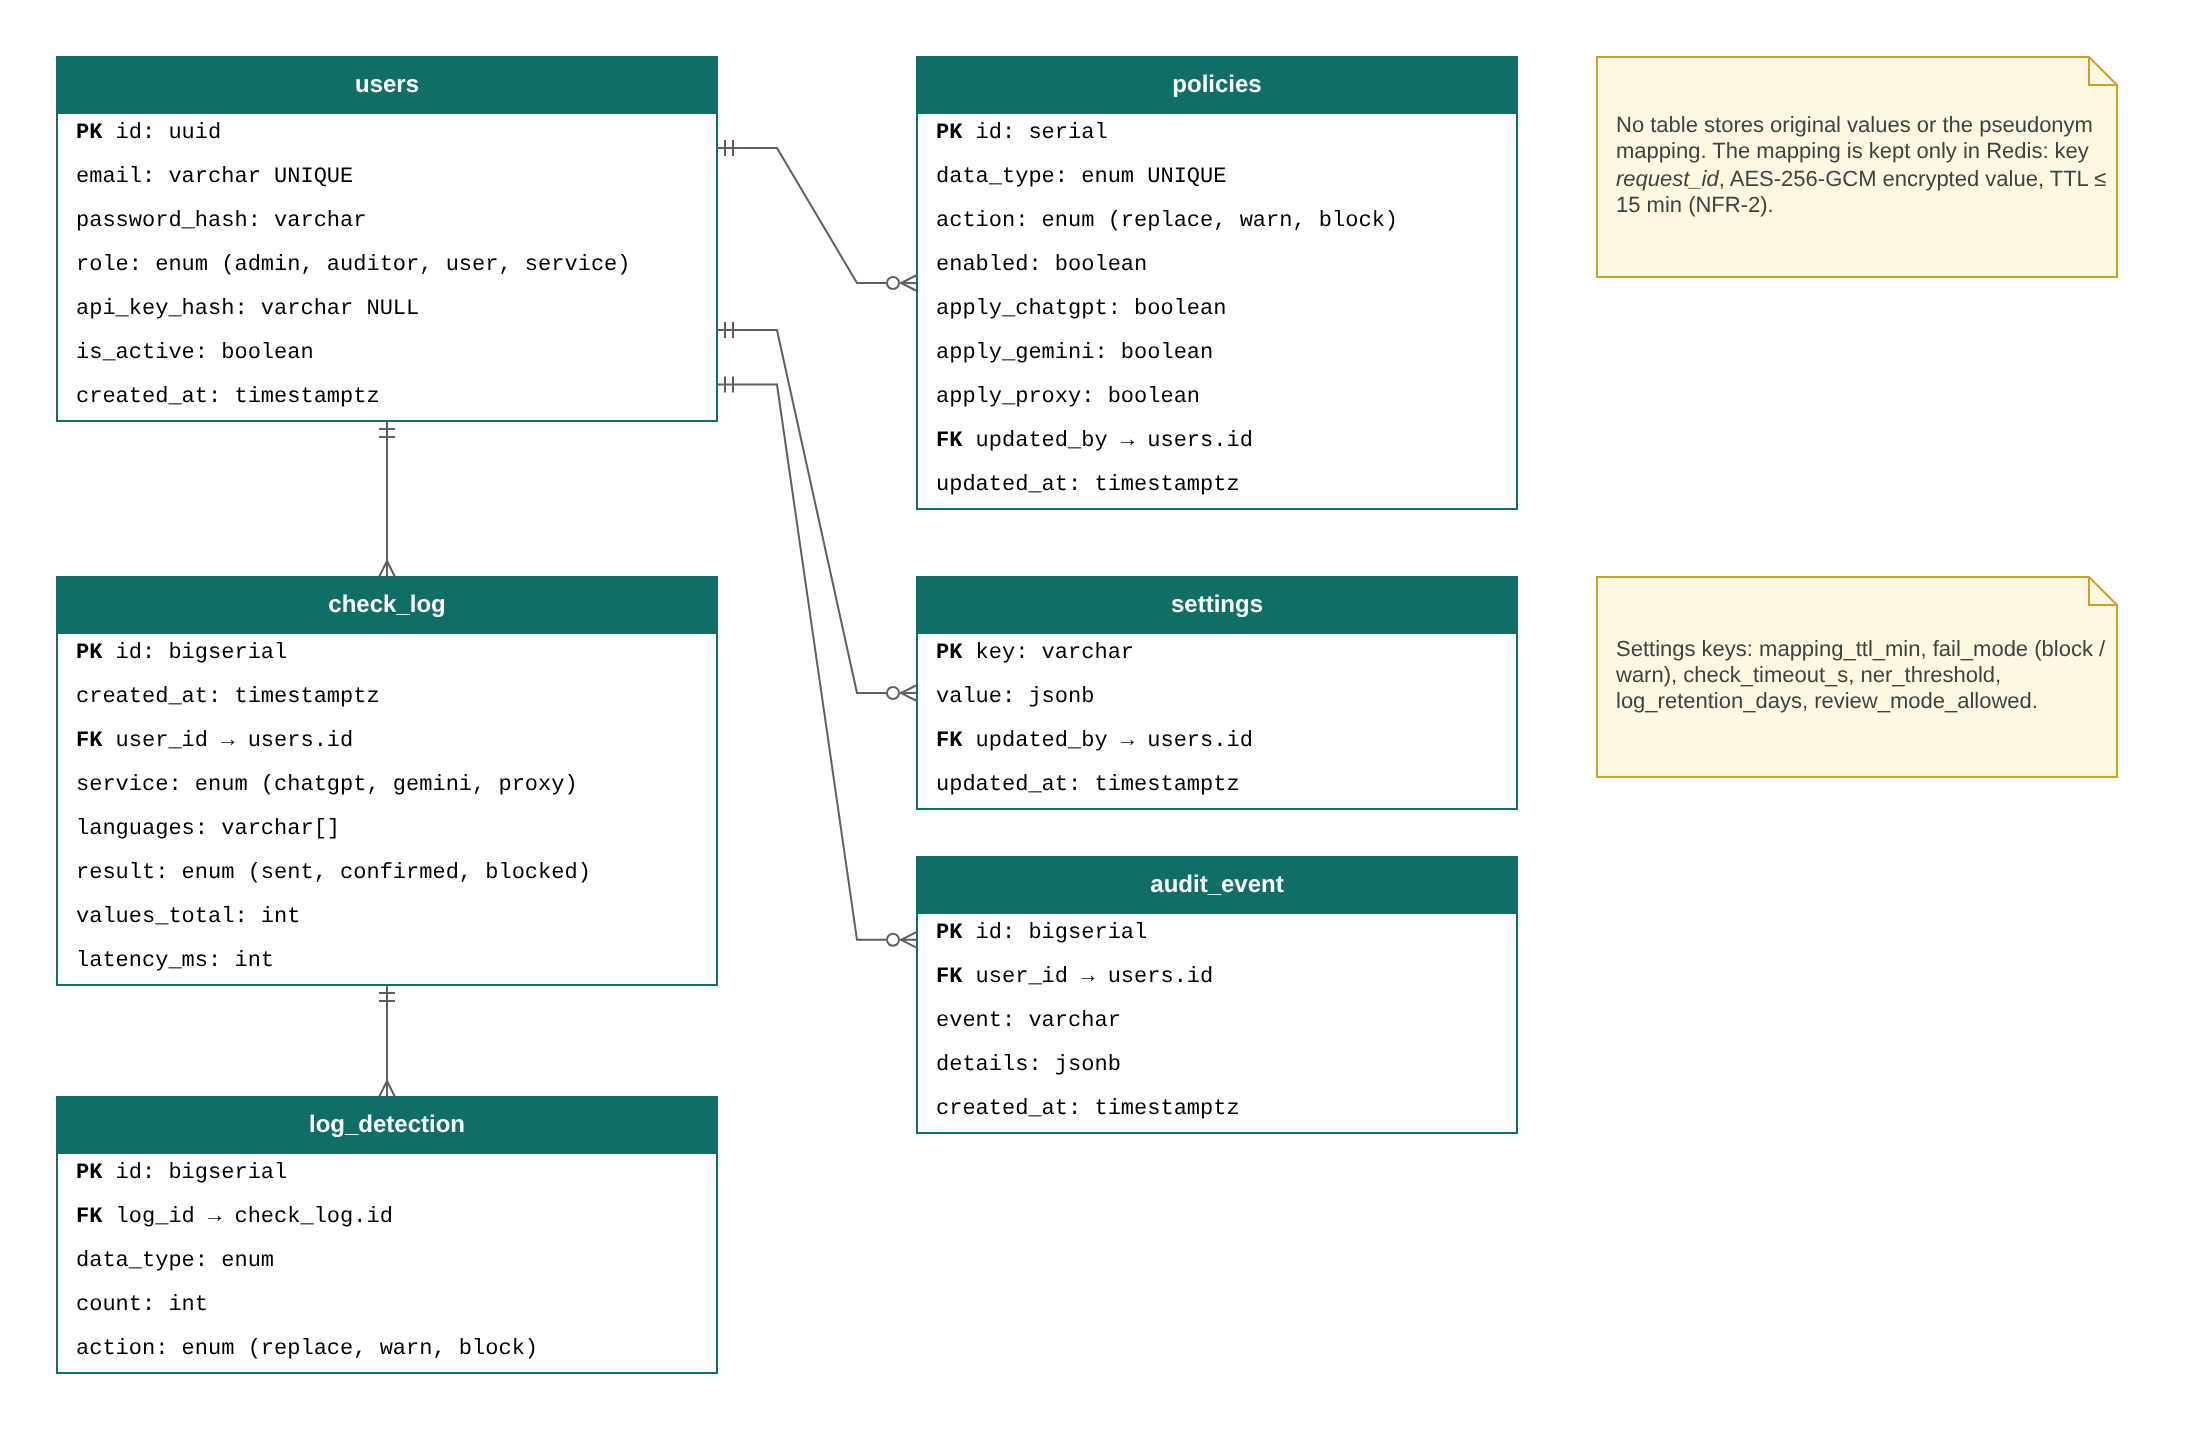
\includegraphics[width=\linewidth]{er-diagram.png}
\caption{Entity-relationship diagram of the database}\label{fig:er}
\end{figure}

The table \texttt{users} stores accounts of all roles, including service accounts with a hashed API key. The table \texttt{policies} contains one record per data type with the selected action and the services to which it applies (FR-6). The table \texttt{settings} stores system parameters such as the mapping retention period, the behaviour on failure and the NER confidence threshold (FR-7.5). Each check is recorded in \texttt{check\_log}, and the number of detected values of each type in \texttt{log\_detection} (FR-7.1). Changes made by administrators are recorded in \texttt{audit\_event}. No table contains original values or the pseudonym mapping: the mapping is stored only in Redis and is deleted automatically (NFR-2).

\end{document}
